\documentclass[border=4pt]{standalone}
\usepackage{amsmath,amssymb,amsfonts}
\usepackage{xcolor,colortbl,array,booktabs,multirow}
\usepackage{tikz}
\usepackage{pgfplots}
\pgfplotsset{compat=1.16}
\usetikzlibrary{arrows, automata, backgrounds, calendar, chains, decorations,
    matrix, mindmap, patterns, petri, positioning, shadows, shapes.geometric,
    trees, shapes, decorations.pathreplacing, calc, tikzmark, arrows.meta,
    intersections, fit, graphs, quotes, angles, decorations.markings}
\newcommand{\st}{\text{ s.t. }}
\newcommand{\x}{\mathbf{x}}
\renewcommand{\b}{\mathbf{b}}
\renewcommand{\c}{\mathbf{c}}
\newcommand{\A}{\mathbf{A}}
\newcommand{\y}{\mathbf{y}}
\newcommand{\z}{\mathbf{z}}
\newcommand{\R}{\mathbb{R}}
\newcommand{\RR}{\mathbb{R}}
\newcommand{\Z}{\mathbb{Z}}
\newcommand{\ZZ}{\mathbb{Z}}
\newcommand{\npcomplete}{NP-complete}
\providecommand{\true}{\text{TRUE}}
\providecommand{\false}{\text{FALSE}}
\tikzset{vertex/.style={circle,fill=black!25,minimum size=20pt,inner sep=0pt},
    edge/.style={draw,thick,-},weight/.style={font=\small},
    selected vertex/.style={vertex, fill=red!24},
    selected edge/.style={draw,line width=2pt,-,red!50},
    ignored edge/.style={draw,line width=2pt,-,black!20}}
\newcommand{\vect}{\vec}
\providecommand{\ds}{\displaystyle}
\providecommand{\longvect}{\overrightarrow}
\usepackage[normalem]{ulem}
\definecolor{ocre}{RGB}{243,102,25}
\providecommand{\leftB}{\left[}
\providecommand{\rightB}{\right]}
\tikzset{directed/.style={postaction={decorate,decoration={markings,mark=at position .65 with {\arrow{>}}}}},
    directed1/.style={postaction={decorate,decoration={markings,mark=at position .65 with {\arrow{>}}}}}}
\begin{document}
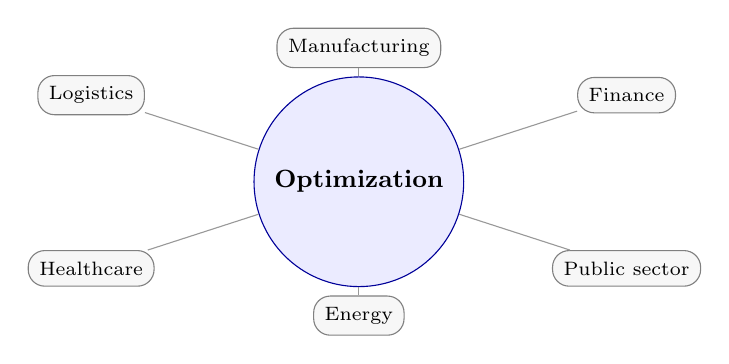
\begin{tikzpicture}[
  hub/.style={draw=blue!60!black, fill=blue!8, circle, font=\small\bfseries, inner sep=6pt},
  sec/.style={draw=black!50, rounded corners=6pt, fill=black!3, font=\scriptsize, inner sep=4pt},
  sp/.style={draw=black!40}]
  \node[hub] (c) at (0,0) {Optimization};
  \node[sec] (a) at (-3.4,1.1) {Logistics};
  \node[sec] (b) at (0,1.7) {Manufacturing};
  \node[sec] (f) at (3.4,1.1) {Finance};
  \node[sec] (h) at (-3.4,-1.1) {Healthcare};
  \node[sec] (e) at (0,-1.7) {Energy};
  \node[sec] (g) at (3.4,-1.1) {Public sector};
  \foreach \n in {a,b,f,h,e,g} \draw[sp] (c) -- (\n);
\end{tikzpicture}
\end{document}
